\documentclass[a4paper,12pt]{report}

\usepackage{alltt, fancyvrb, url}
\usepackage{graphicx}
\usepackage[utf8]{inputenc}
\usepackage{float}
\usepackage{hyperref}
\usepackage[italian]{babel}
\usepackage{appendix}
\usepackage[italian]{cleveref}

\title{RELAZIONE PROGETTO DI PROGRAMMAZIONE AD OGGETTI}
\author{Margherita Balzoni, Chiara Castiglioni, Edoardo Desiderio, \\Virginia Foschi, Simone Ruggeri}
\date{Febbraio 2023}

\begin{document}
\maketitle
\titlepage
\tableofcontents
\newpage

\chapter{Analisi}
Il seguente capitolo contine l'analisi dei requisiti e del problema, ovvero fornisce una descrizione del dominio applicativo e delle funzionalità offerte dall'applicazione.
\section{Requisiti}
Il progetto, commissionato dall'Università di Bologna\footnote{\url{https://www.unibo.it/it}}, si pone come obbiettivo la realizzazione di un videogioco del genere Arcade, di nome Arkanoid\footnote{\url{https://it.wikipedia.org/wiki/Arkanoid}}.\\L'obbiettivo del gioco è quello di superare i tre round per ogni livello di difficoltà cercando di totalizzare un punteggio elevato, abbattendo un certo numero di mattoncini colorati colpendoli con una sfera.
\\
\subsection*{Requisiti funzionali}
\begin{itemize}
    \item Menù principale che all'avvio del software permette di scegliere il livello in base alla difficoltà e visionare la classifica.
    \item L’applicazione implementa la fisica della palla e ne gestisce il rimbalzo con i bordi dell’arena, con il pad e con i mattoncini.
    \item Area di gioco composta da un certo numero di mattoncini che cambiano disposizione ad ogni livello.
    \item Gestione dei parametri del giocatore, in particolare vita (che diminuisce ogni volta che il pad non colpisce la pallina) e il punteggio.
    \item Organizzazione del gioco a livelli, ciascuno composto da 3 round ciascuno
    \item Creazione di differenti bonus o malus
    \item Avanzamento del gioco con difficoltà incrementale (quantità di mattoncini aumentata per ogni round)
    \item Realizzazione e aggiornamento di una classifica basata sul punteggio del giocatore
          \subsection*{Requisiti non funzionali}
    \item Fluidità del movimento degli oggetti
    \item Grafica user-friendly
\end{itemize}
\section{Analisi e modello del dominio}
Il gioco è strutturato a livelli di difficoltà crescente, ognuno dei quali presenta una diversa disposizione composta da tre diverse tipologie di mattoncini. Ogni livello è composto da tre round dove vi è sempre più un numero crescente di mattoncini.
Il livello contiene anche informazioni riguardanti il punteggio, il quale incrementa man mano che i mattoncini vengono distrutti e la vita del giocatore.
\\Le vite stabiliscono il numero di tentativi che l'utente ha per superare il livello al termine delle quali il giocatore potrà segliere se salvare il proprio punteggio, tornare alla schermata di gioco oppure uscira dall'applicazione, le stesse scelte saranno disponibili anche in caso di vittoria.
\\Il giocatore ha a disposizione un pad che si può muovere solo orrizzontalmente con il quale potrà far rimbalzare la sfera contro i mattoncini.
Le tre tipologie di mattoncini sono:
\begin{itemize}
    \item NormalBrick: mattoncini normali che se colpiti una volta dalla palla vengono distrutti.
    \item HardBrick: mattoncini che devono essere colpiti due volte per essere distrutti.
    \item Obstacle: mattoncini indistruttibili.
\end{itemize}
Ulteriori dettagli circa le entità presenti possono essere consultati attraverso la \Cref{images:analysis} inserita di seguito.
\begin{figure}[H]
    \centering{}
    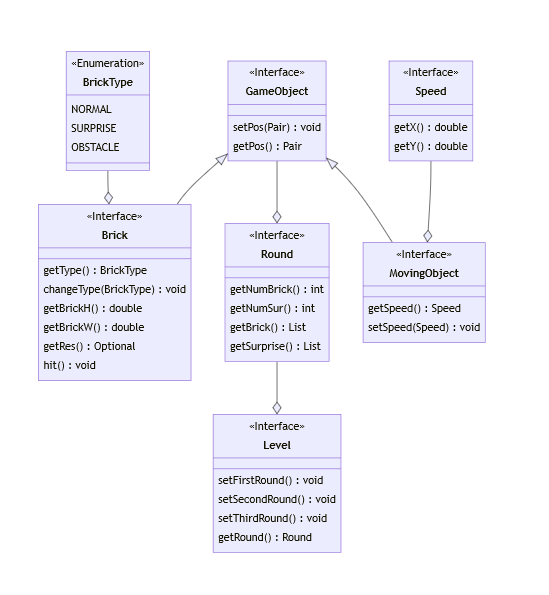
\includegraphics{images/analysis.png}
    \caption{Schema UML dell'analisi del problema, con rappresentate le entità principali ed i rapporti fra loro}
    \label{images:analysis}
\end{figure}
\chapter{Design}
\section{Architettura}
Si è optato per un pattern architetturale ispirato a un MVC(Model , View, Controller) in cui ci siamo impegnati il più
possibile a mantenere separati gli aspetti logici, di controllo e di grafica. Tuttavia non ne rispetta tutti i principi poiché nella classe GameEngine ci siamo
serviti di una funzionalità di una libreria grafica (SwingWorker).
\\La nostra strategia ha comunque il vantaggio che qualora fosse necessario cambiare l'interfaccia grafica
questo non causerebbe modifiche nelle classi di Model e Controller.
\section{Desing dettagliato}
\chapter{Sviluppo}
\section{Testing automatizzato}
\section{Metodologia di lavoro}
\section{Note di sviluppo}
\chapter{Commenti finali}
\section{Autovalutazione e lavori futuri}

\appendix
\section{Guida utente}



\end{document}
